%! Licence = CC BY-NC-SA 4.0

%! Author = gianfluetsch
%! Date = 30. Dez 2021
%! Project = cydef_summary

\section{Red Teaming}
Red Team führt realitätsnahe Cyber-Angriffe gegen Kunden Infrastruktur und Dienste durch. Es versetzt sich in die \textbf{Denk} und \textbf{Handlungsweise} eines Gegners, um dadurch \textbf{neue Erkenntnisse} über die \textbf{eigenen Schwächen} zu erlangen und \textbf{mitigierende Massnahmen} einleiten zu können.

\subsection{Audit/Pen Testing vs. Red Teaming}
\begin{itemize}
    \item Beim \textbf{Pen-Testing} ist der Fokus mehr auf einem spezifischen System/ Komponenten
    \begin{itemize}
        \item Gain \textbf{overview} of vulnerabilities
        \item Scope \& budget \textbf{depend on project}
        \item Focus on \textbf{efficiency} (no exploitation)
        \item Part of \textbf{secure development lifecycle}\\
    \end{itemize}
    \item Beim \textbf{Red Teaming} ist man freier und versucht verschiedene Systeme anzugreifen und via Lateral Movement von einem System auf ein anderes zu kommen (höchstes Ziel $\rightarrow$ Active Directory)
    \begin{itemize}
        \item Test \textbf{resilience} (Wiederstandsfähigkeit) agains real attacks
        \item \textbf{Independent} and adaptable attacks
        \item Focus on \textbf{crown jewels} (exploitation)
        \item Periodical cases, ad-hoc
    \end{itemize}
\end{itemize}

\subsection{Blue Teaming vs. Red Teaming}
\begin{center}
    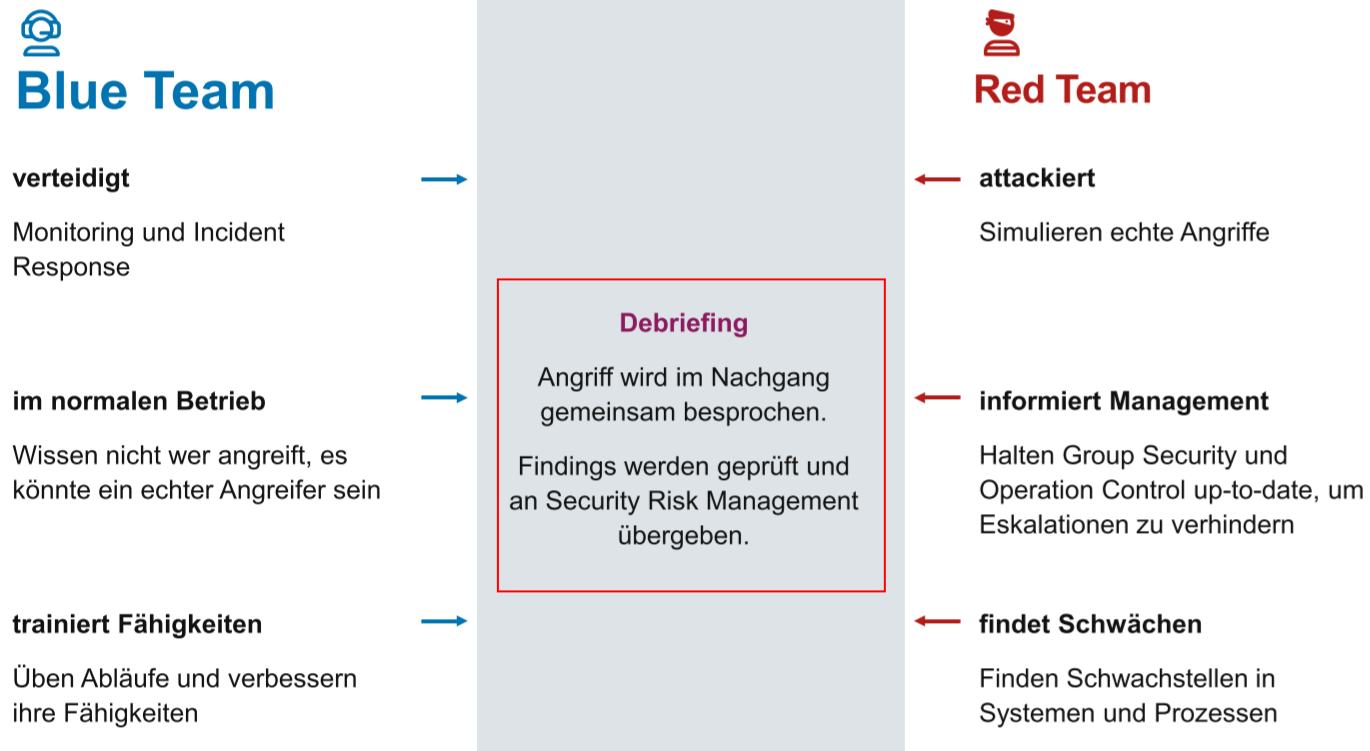
\includegraphics[width=1.0\linewidth]{./img/14-red_teaming/blue_red}
    \vspace{-8pt}
\end{center}

\subsection{Code of Conduct}
\begin{itemize}
    \item keine absichtlichen Störungen (Down Times) oder SLA Impact herbeiführen
    \item kein absichtlicher Zugriff (lesend oder verändernd) auf Kundendaten
    \item keine absichtlichen destruktiven Aktionen durchführen
    \item bestehende Sicherheitsmassnahmen werden nicht geschwächt oder ausser Betrieb genommen (z.B. keine Any-Any FW-Rules erstellen, keine Admin Accounts mit Admin/Admin anlegen, etc.)
    \item Findings werden geschützt und nur mit Personen geteilt die ein need to know haben
\end{itemize}

\columnbreak

\subsection{Kerberoasting}
Get service ticket for user/service with SPN set and crack its password
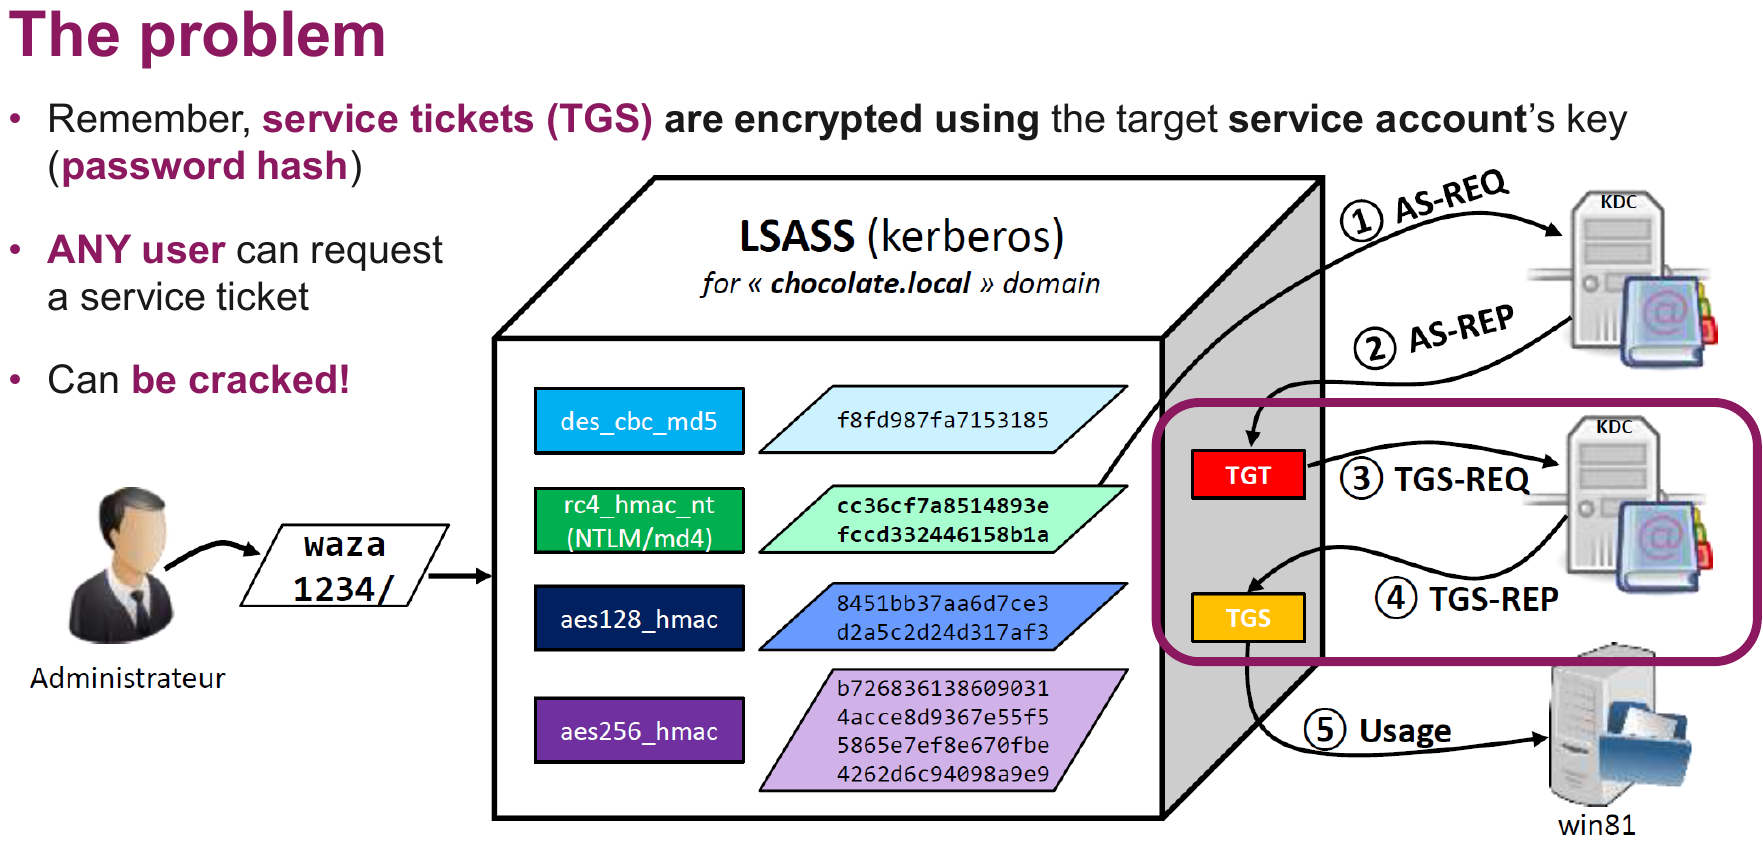
\includegraphics[width=\linewidth]{./img/14-red_teaming/kerberoasting}
\begin{enumerate}
    \item Find a user/service account (rather than a machine account) with a service principal name (SPN) set
    \item Request a service ticket with RC4\_HMAC\_MD5 encryption and extract a hash from it
    \item Attempt to crack the user's password using hashcat or John the Ripper
\end{enumerate}
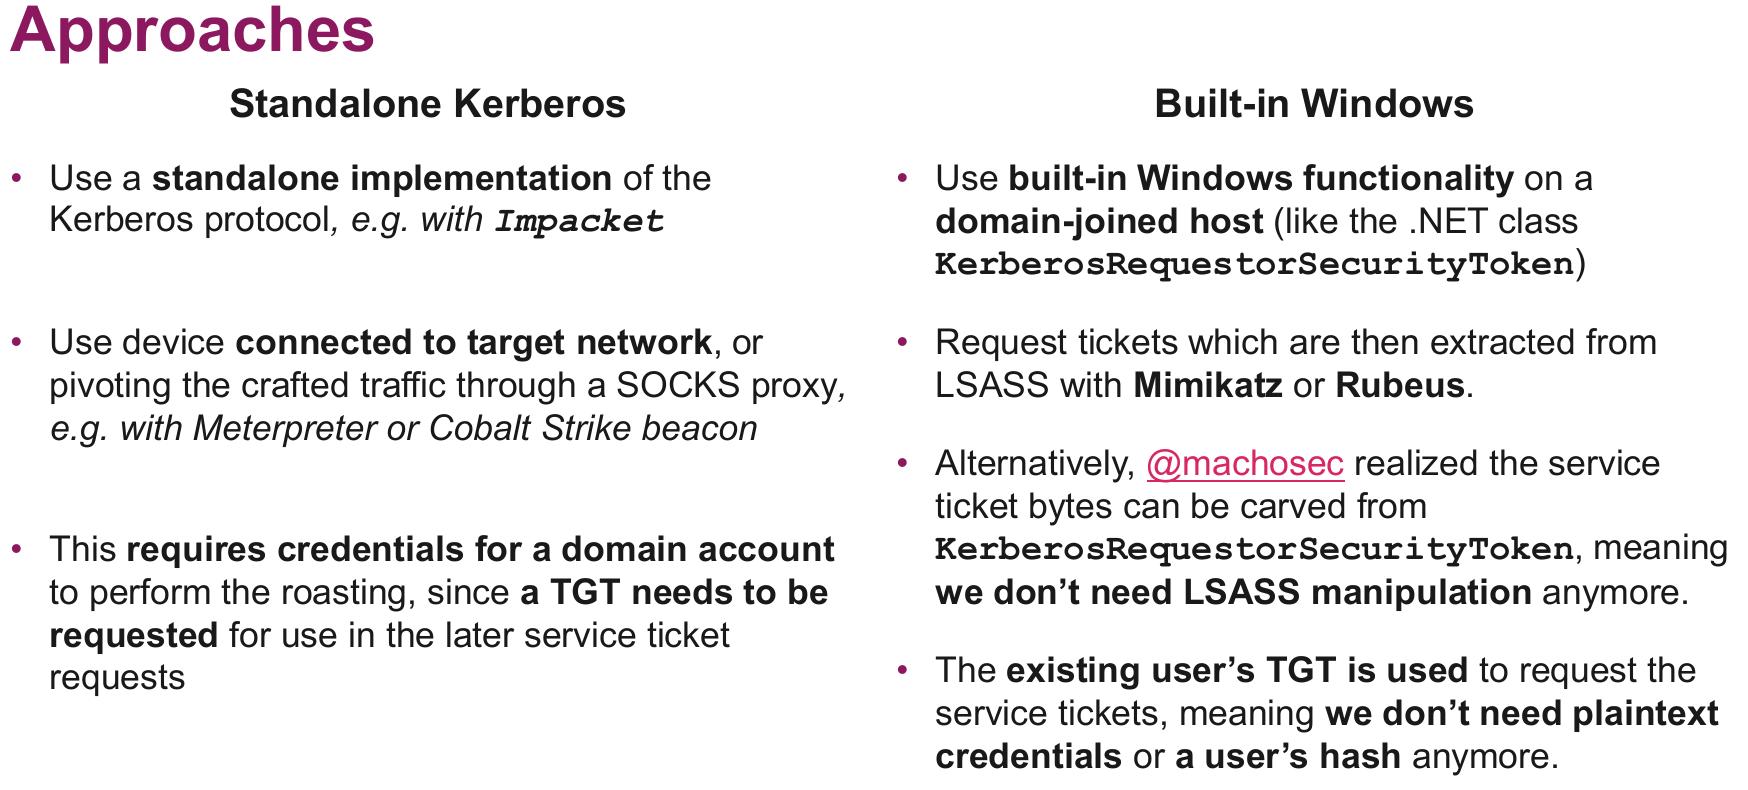
\includegraphics[width=\linewidth]{./img/14-red_teaming/kerberos_tgt}

\subparagraph{Red Teaming}
\subsection{Step 1: Host \& Service Discovery}
Das Netzwerk soll gescannt werden, dass man weiss was im Netz ummen ist, wselche Ports offen sind, Hostnames.
Explizit wird ein Service Discovery Scan gemacht, um genauere oder weiterführende Infos zu erhalten. 

\begin{lstlisting}[language=bash]
    ip -c address list eth0
    nmap -n -sn 10.0.1.0/24 -oA host_discovery --min-rate=20000
    cat host_discovery.gnmap | awk '/Up/ {print $2}' | sort -Vu > hosts.txt
    nmap -n -sC -sV -iL hosts.txt -oA script_version_scan --min-rate=20000
\end{lstlisting}

\subsection{Step 2: Situational Awareness \& Privilege Escalation on Windows 10 Client}
Nachdem die Verbindung zu einem Client (z.B. über RDP) hergestellt wurde, müssen möglichst viele Informationen gesammelt werden. Das Ziel ist es, sich über die verfügbaren Angriffsflächen und über mögliche Optionen zur Ausweitung der Privilegien bewusst zu werden.

Zu diesem Zeitpunkt hat man oft noch keine lokalen Admin-Rechte und versucht nun mit verschiedenen Tools diese zu erlangen.

\subsubsection{Powersploit}

\paragraph{Begriffe}

\begin{itemize}
    \item Privsec module
\end{itemize}

\paragraph{Privilege Escalation}
\begin{enumerate}
    \item Invoke-AllChecks gibt alle sMöglichkeitne zur Privilege Escalation aus
    \item AlwaysInstallElevated - der funktioniert fast immer. hijackable dll aber meist nicht.
    \item Write-UserAddMSI - MSI erstellen um AlwasInstalleElevated Registry Key ausführen -> zum exploiten. *erstellt user mit gruppe die man dann brauchen kann*
    ^^ den kann man bruachen um mit MSI user zu erstellen/als admin auszuführen. "bakennte schwachstelle". * mit dem key sagt man, dass wenn man dieses MSI ausführt, es immer als Admin ausgeführt werden soll* 
    \item \textbf{ab jetzt lokaler admin}
    \item \lstinline|UserAdd.msi| ausführen mit den \textit{bypass / Privilege Escalation} Rechten um User zu erstellen $\rightarrow$ \textbf{Membership ist Administratoren}.
\end{enumerate}

\paragraph{Commands}
\begin{itemize}
    \item powershell -exec bypass
    \begin{itemize}
        \item execution policy überspringen
    \end{itemize}
    \item Import\-Module .\\Privesc.psd1
    \begin{itemize}
        \item wichtiges Privsec Module importieren
    \end{itemize}
    \item Invoke-AllChecks
    \begin{itemize}
        \item Privilege Escalation laufen lassen
        \item Output:
    \end{itemize}
\end{itemize}


\begin{lstlisting}[language=bash]
    ModifiablePath    : C:\Users\tmassie\AppData\Local\Microsoft\WindowsApps
    IdentityReference : winattacklab\tmassie
    Permissions       : {WriteOwner, Delete, WriteAttributes, Synchronize...}
    %PATH%            : C:\Users\tmassie\AppData\Local\Microsoft\WindowsApps
    Name              : C:\Users\tmassie\AppData\Local\Microsoft\WindowsApps
    Check             : %PATH% .dll Hijacks
    AbuseFunction     : Write-HijackDll -DllPath 'C:\Users\tmassie\AppData\Local\Microsoft\WindowsApps\wlbsctrl.dll'

    Check         : AlwaysInstallElevated Registry Key
    AbuseFunction : Write-UserAddMSI

    UnattendPath : C:\windows\Panther\Unattend.xml
    Name         : C:\windows\Panther\Unattend.xml
    Check        : Unattended Install Files
\end{lstlisting}

\paragraph{Kurz \& Knapp}\mbox{} \\
Den kann man brauchen um mit \textit{MSI} User zu erstellen/ als admin auszuführen (bakannte Schwachstelle). \textbf{Mit dem Key sagt man, dass wenn man dieses \textit{MSI} ausführt, es immer als Admin ausgeführt werden soll}.
$\rightarrow$ das Tool brauchen um an lokale Adminrechte zu kommen, um dann mit Mimikatz Domänen-Admin Credentials zu bekommen.

\subsection{Step 3: AD Information Gathering \& Analysis}

\subsubsection{Pingcastle}
PingCastle ist ein Tool zur schnellen Analyse des Sicherheitsniveaus des Active Directory. Es handelt sich um eine Methodik, die auf einer Risikobewertung und einem Reifegradrahmen basiert. Es wird zwar nicht jede einzelne Schwachstelle oder Fehlkonfiguration aufdecken, aber es sollte Ihnen ein gutes Gesamtbild der Sicherheitslage Ihres ADs vermitteln.
\begin{itemize}
    \item Health Check des AD
    \item Mit Bloodhound Resultate analyseieren
\end{itemize}

\subsubsection{Bloodhound}
BloodHound nutzt die Graphentheorie, um die versteckten und oft unbeabsichtigten Beziehungen innerhalb einer Active Directory-Umgebung aufzudecken. Angreifer können mit BloodHound auf einfache Weise hochkomplexe Angriffspfade identifizieren, die andernfalls nicht schnell zu erkennen wären. Verteidiger können mit BloodHound dieselben Angriffswege identifizieren und eliminieren. Sowohl blue als auch red Teams können BloodHound nutzen, um auf einfache Weise ein tieferes Verständnis der Berechtigungsbeziehungen in einer Active Directory-Umgebung zu erlangen.BloodHound besteht aus zwei Teilen:Der GUI zur Analyse der gesammelten Daten (eigentlich BloodHound genannt).Die Tools zum Sammeln von Daten aus dem AD (auch als Collector oder Ingestor bezeichnet). Sie sind in verschiedenen Varianten verfügbar (PowerShell, .NET, ...)

BloodHound bietet Ihnen verschiedene Möglichkeiten, die gesammelten Daten zu analysieren und mit ihnen zu interagieren. Sie können entweder alle gesammelten Objekte (wie Computer, Benutzer, Gruppen usw.) durchsuchen, die integrierten Abfragen zum Abrufen von Daten verwenden oder Ihre eigenen Abfragen definieren. Es sieht, wie wann wer mit RDP wohin zugegriffen hat, welche Gruppen, Memberhships usw.** Man kann das Ziel(z.B. DB-Server im Netz) angeben wo man hin will, dann zeigt es auf - basierend auf den Angaben wo man schon im Netz kontrolle hat - man am Besten dorthin kommt. Wie ein Navi, mit Voraussetzungen was man haben muss um irgendwo hinzukommen.** Typen der Devices die man manuell setzen kann: owned \& high value target

Bloodhound kann weiterhin verwendet werden, um eine Übersicht über alle kompromitierten Systeme zu erhalten. Dabei kann nun jeweils das neu übernommene System/ Account als "owned" markiert werden und Bloodhound kann so neue Angriffsmöglichkeiten/ Angriffswege berechnen.

\paragraph{Ausführen}\mbox{} \\
Auf einem AD gejointem Client

\begin{lstlisting}[language=PowerShell]
    # ergibt ein ZIP
    > .\SharpHound.exe -c All,GPOLocalGroup

    - Resolved Collection Methods: Group, Sessions, LoggedOn, Trusts, ACL, ObjectProps, LocalGroups, SPNTargets, Container, GPOLocalGroup
    ...
    Status: 106 objects finished (+106 26.5)/s -- Using 30 MB RAM
    Enumeration finished in 00:00:04.6680493
    Compressing data to .\20200909103934_BloodHound.zip    
\end{lstlisting}

Daten können nun im Bloodhound GUI anschauen
\begin{itemize}
    \item zeigt alle Abhängigkeiten im AD auf
    \item \textbf{man kann angeben was man schon owned, dann werden die möglichen Angriffe aufgezeigt und auf was man los soll}\\
\end{itemize}

\subsection{Step 4: Credential Dumping on Windows 10 Client}
Wenn Sie über lokale administrative Rechte auf einem Windows-Rechner verfügen, können Sie dies missbrauchen, um verschiedene Formen von Anmeldeinformationen abzurufen, die auf dem jeweiligen Rechner gespeichert sind. Dazu gehören Anmeldedaten lokaler Benutzerkonten (die in der SAM-Datei gespeichert sind) sowie vorübergehend zwischengespeicherte Anmeldedaten aktuell angemeldeter Benutzer (die im Speicher des lsass-Prozesses gehalten werden).\\

\begin{itemize}
    \item Run as Admin mit dem neu selbst gemachten User aus der Aufgabe von vorhin
    \item privilege::debug - um Lsass Credentials zu droppen
    \item log my\_log.txt - logging aktivieren
    \item sekurlsa::logonpasswords - \textbf{effektive Credentials auslesen}\\
\end{itemize}

\begin{lstlisting}[language=bash]
    Authentication Id : 0 ; 6453349 (00000000:00627865)   
    Session           : Interactive from 2
    User Name         : backdoor
    Domain            : Client1
    Logon Server      : Client1
    Logon Time        : 11/12/2021 4:46:23 PM
    SID               : S-1-5-21-1681067654-3552921923-1543340101-1005
        msv :
         [00000003] Primary
         * Username : backdoor
         * Domain   : Client1
         * NTLM     : a9fdfa038c4b75ebc76dc855dd74f0da
         * SHA1     : 9400ae28448e1364174dde269b2cce1bca9d7ee8
    [CUT]
\end{lstlisting}

\begin{itemize}
    \item token::elevate - \textbf{Credentials auslesen des lokalen SAM}
    \item lsadump::elevate - \textbf{Permissions elevaten}
    \begin{itemize}
        \item process token: token für user auf mascine
        \item thread token: token für NT Auth/System, Maschine
    \end{itemize}
    \item lsadump::sam - \textbf{SAM Database mit NTLM und so dumpen}
\end{itemize}

\begin{lstlisting}[language=bash]
    Domain : Client1
    SysKey : 2d102d4d76b467c3aa870e40d01a3f55
    Local SID : S-1-5-21-1681067654-3552921923-1543340101

    SAMKey : d777e5a8096311cf0c6dd57edebad324

    RID  : 000001f4 (500)
    User : lab_admin
    Hash NTLM: f6e934388fc080ee870bd0637e4992f9
    [CUT]
\end{lstlisting}

Logs anschauen, da ist vieles drin wie username, dmain, credentials, UND NTLM HASHES, die sind am wichtigsten. kann für pass the hash attacken genutzt werden



\subsection{Step 5A: Lateral Movement to FS1 via Domain User}
In den vorangegangenen Übungen konnten wir uns lokale Administratorrechte auf dem Windows 10-Client verschaffen und anschließend alle auf diesem Rechner gespeicherten Anmeldeinformationen auslesen. Die gesammelten Daten enthielten unter anderem den NTLM-Hash des Domänenbenutzers "aalfort", der lokaler Administrator auf dem Rechner FS1.winattacklab.local ist.

Diese Konstellation kann nun missbraucht werden, um mit einer Technik namens "pass-the-hash" seitlich auf FS1.winattacklab.local zu gelangen.\\

$\rightarrow$ Python Script für pass the hash attacken: \lstinline|psexec.py|\\

\begin{enumerate}
    \item psexec.py - python zum NTLM Hash probieren
    \item \textbf{psexec.py  -hashes :9859340265d3b3c1eb628ece70ebc238 winattacklab.local/aalfort@10.0.1.101}\\
\end{enumerate}

\begin{lstlisting}[language=PowerShell]
    Impacket v0.9.22.dev1+20200819.170651.b5fa089b - Copyright 2020 SecureAuth Corporation

    [*] Requesting shares on 10.0.1.101.....
    [*] Found writable share ADMIN$
    [*] Uploading file LZzQLrwi.exe
    [*] Opening SVCManager on 10.0.1.101.....
    [*] Creating service HIbO on 10.0.1.101.....
    [*] Starting service HIbO.....
    [!] Press help for extra shell commands
    Microsoft Windows [Version 10.0.17763.1397]
\end{lstlisting}

\subsection{Step 5B: Lateral Movement to FS1 via Local User}
Wir werden nun lernen, wie wir überprüfen können, ob dieser lokale Benutzer auch auf anderen Rechnern existiert. Wenn dies der Fall ist UND der Benutzer das gleiche Passwort hat, kann dies missbraucht werden, um mit einer Technik namens "pass-the-hash" seitlich auf das/die andere(n) System(e) zu gelangen.

Mit dem NTLM-Hash des Helpdesk-Benutzers können wir nun mit einem Tool namens \textbf{CrackMapExec} leicht überprüfen, ob dasselbe lokale Benutzerkonto (mit demselben Passwort) auf anderen Systemen existiert.\\

$\rightarrow$ Python Script für pass the hash attacken: \lstinline|psexec.py|\\

\begin{enumerate}
    \item psexec.py - python zum NTLM Hash probieren
    \item \textbf{psexec.py  -hashes :9859340265d3b3c1eb628ece70ebc238 winattacklab.local/aalfort@10.0.1.101}
\end{enumerate}

\begin{lstlisting}[language=PowerShell]
    Impacket v0.9.22.dev1+20200819.170651.b5fa089b - Copyright 2020 SecureAuth Corporation

    [*] Requesting shares on 10.0.1.101.....
    [*] Found writable share ADMIN$
    [*] Uploading file LZzQLrwi.exe
    [*] Opening SVCManager on 10.0.1.101.....
    [*] Creating service HIbO on 10.0.1.101.....
    [*] Starting service HIbO.....
    [!] Press help for extra shell commands
    Microsoft Windows [Version 10.0.17763.1397]
\end{lstlisting}

\subsubsection{CrackMapExec}
Mit dem NTLM-Hash des Helpdesk-Benutzers können wir nun mit einem Tool namens CrackMapExec leicht überprüfen, ob dasselbe lokale Benutzerkonto (mit demselben Passwort) auf anderen Systemen existiert.



\subsection{Step 6: Situational Awareness on FS1}
Wir haben nun Zugriff auf den Host FS1.winattacklab.local mit administrativen Rechten erhalten. Das bedeutet, dass wir nicht mehr nach lokalen Methoden zur Privilegienerweiterung suchen müssen. Stattdessen ist das Ziel, andere wertvolle Informationen zu finden, die uns helfen könnten, andere Benutzer oder Hosts zu kompromittieren.

\subsubsection{Acquiring the Necessary Tools}

\paragraph{PrivescCheck}\mbox{} \\
Dieses Skript zielt darauf ab, häufige Windows-Konfigurationsprobleme aufzuzählen, die zur lokalen Privilegienerweiterung ausgenutzt werden können. Außerdem sammelt es verschiedene Informationen, die für eine Ausnutzung und/oder Nachnutzung nützlich sein könnten.
Dieses Tool soll Sicherheitsberatern dabei helfen, potenzielle Schwachstellen auf Windows-Rechnern während Penetrationstests und Workstation/VDI-Audits zu identifizieren. Es ist nicht für den Einsatz bei Red-Team-Einsätzen gedacht, kann aber dennoch viele nützliche Informationen liefern.

\subparagraph{Lines of Interest in output}\mbox{} \\

\begin{lstlisting}[language=bash]
    | KO | Med. | CREDS > Unattend Files -> 1 result(s)       |
\end{lstlisting}

Dies zeigt an, dass eine Datei für die unbeaufsichtigte Installation gefunden wurde, die oft Anmeldeinformationen enthält. Wenn Sie in der Ausgabe ein wenig nach oben scrollen, sollten Sie die Details zu diesem Fund finden:

\begin{lstlisting}[language=bash]
    +------+------------------------------------------------+------+

    | TEST | CREDS > Unattend Files                         | VULN |

    +------+------------------------------------------------+------+

    | DESC | Locate 'Unattend' files and check whether they        |

    |      | contain any clear-text credentials.                   |

    +------+-------------------------------------------------------+

    [*] Found 1 result(s).
    Type     : LocalAccount
    Domain   : N/A
    Username : admin
    Password : Winter2019
    File     : C:\Windows\Panther\Unattend.xml
\end{lstlisting}

PrivescCheck die Datei direkt geparst und das Passwort \textcolor{red}{\textit{Winter2019}} für den Benutzer \textcolor{red}{\textit{admin}} gefunden.

\subparagraph{unattend.xml}\mbox{} \\
Antwortdateien (oder Unattend-Dateien) können verwendet werden, um Windows-Einstellungen in Ihren Images während der Einrichtung zu ändern. Sie können auch Einstellungen erstellen, die Skripte in Ihren Images auslösen, die ausgeführt werden, nachdem der erste Benutzer sein Konto erstellt und seine Standardsprache ausgewählt hat.



\subsection{Step 7: Password Spraying}
Auf dem Host FS1 konnten wir eine Datei abrufen, die ein Kennwort enthielt. Das Kennwort lautete "Winter2019", was einem Standardkennwort sehr ähnlich sieht, wie es von einem Servicedesk beim Zurücksetzen eines Kennworts vergeben werden könnte.
Eine gängige Angriffstechnik besteht darin, dieses Passwort nun für alle Benutzer innerhalb der Domäne zu verwenden. Dies wird als "Passwort-Spraying" bezeichnet.

\subsubsection{Automate Passwort Spraying}
Es gibt eine Vielzahl von Tools, mit denen sich das Sprühen von Kennwörtern automatisieren lässt. Einige Tools stellen eine direkte Verbindung zum Active Directory her, um eine Liste aller Benutzer abzurufen, bei anderen müssen Sie diese Informationen selbst bereitstellen.
In diesem Fall werden wir ein Tool namens \textcolor{red}{\textit{kerbrute}} verwenden, das eine Benutzerliste benötigt.

\subsubsection{Checking the Password Lockout Policy}
Ein wichtiger Punkt bei der Durchführung von Passwort-Spraying ist, dass Benutzerkonten nicht wegen zu vieler fehlgeschlagener Anmeldungen gesperrt werden dürfen

\subsubsection{Password Spraying vs. Brute-Force}
Beim Password Spraying wird das gleiche Passwort bei verschiedenen Benutzern getestet. Das Passwort bleibt also gleich, aber die Benutzernamen wechseln.
Bei einem Brute-Force Angriff bleibt der Benutzername gleich und verschiedene Passwörter werden verwendet.

Mit Password Spraying kann oft eine Sperrung des Benutzer-Accounts umgangen werden, da oft nicht überprüft wird von welcher IP-Adresse die Loginversuche kommen.

\subsubsection{Mitigation}
Ein Abwehrmechanismus gegen Password Spraying ist den Zugriff einer IP-Adresse zu blockieren, wenn z.B. mehr als 10 Loginversuche falsch waren (egal mit welchem Username).

Mit einem Tool wie proxychain kann dies aber umgangen werden, da damit die IP-Adresse nach 9 Versuchen via Tor geändert werden kann.

\subsubsection{Bloodhound}
Bloodhound kann weiterhin verwendet werden, um eine Übersicht über alle kompromitierten Systeme zu erhalten. Dabei kann nun jeweils das neu übernommene System/ Account als "owned" markiert werden und Bloodhound kann so neue Angriffsmöglichkeiten/ Angriffswege berechnen.



\subsection{Step 8: Lateral Movement to WS1}
In der vorherigen Aufgabe haben wir erfolgreich die Klartext-Anmeldeinformationen des Benutzers "cclear" abgerufen, der lokaler Administrator des Rechners WS1 ist. Versuchen wir nun, dies zu verifizieren.

\subsubsection{Windows Defender (What is happening in the Background)}
In der realen Welt ist es nicht immer einfach, sich seitlich zwischen Systemen zu bewegen. Vor allem dann nicht, wenn bekannte, öffentlich verfügbare Tools wie die Impacket-Sammlung verwendet werden, da sie von AV-Lösungen recht leicht erkannt werden können. Wenn Sie den vorherigen Schritt ausgeführt haben, hat Windows Defender (das auf WS1 aktiv ist und ausgeführt wird) Ihre Verbindung erkannt und blockiert.\\

Wenn die Verbindung im vorigen Abschnitt hängen geblieben ist, betrachten wir Microsoft Defender als die blockierende Instanz.

\subsubsection{smbclient.py}
Eine bessere Methode zur Überprüfung der Anmeldeinformationen, die wir auf WS1 gefunden haben (via psexec.py), wäre die Verwendung einer weniger "aufdringlichen" Technik, wie z. B. das SMB-Protokoll, speziell das Tool smbclient.py aus der Impacket-Sammlung.\\

Da dies eine normale SMB-Verbindung imitiert, wird auf der WS1 nichts Ungewöhnliches angezeigt, und das Ziel, die Anmeldeinformationen zu überprüfen, wird dennoch erreicht.

\subsubsection{Other means of Verification}
Natürlich sind die oben beschriebenen Methoden zur Überprüfung von Anmeldeinformationen nicht die einzigen. Es gibt viele andere Tools und Techniken, mit denen ein Angreifer überprüfen kann, ob die gesammelten Anmeldeinformationen (sowohl Hashes als auch Passwörter) gültig sind oder nicht. Natürlich sind einige von ihnen heimlicher oder leistungsfähiger als andere. Daher ist es wichtig, dass Sie sich immer überlegen, was Sie erreichen wollen, und das richtige Tool dafür auswählen!

\paragraph{CrackMapExec}\mbox{} \\
Ein sehr leistungsfähiges Tool zur Überprüfung von Anmeldeinformationen für ein oder mehrere Ziele ist CrackMapExec.\\

Mit diesem Tool können Sie ganz einfach (mehrere Sätze von) Anmeldeinformationen für einen einzelnen Host, Ziellisten, IP-Bereiche oder sogar ganze Subnetze prüfen. Es unterstützt mehrere Protokolle wie SSH, SMB, WINRM, LDAP usw. Darüber hinaus kann es auch automatisch Befehle auf Systemen ausführen, bei denen eine erfolgreiche Anmeldung festgestellt wurde.\\

CrackMapExec kann auch verwendet werden, um eine Anmeldung auf mehreren Systemen zu testen. Z.B. können alle Rechner in einem Subnet getestet werden.



\subsection{Step 9: Situational Awareness \& Credential Dumping on WS1}
Wir sind erfolgreich auf den Host WS1 umgezogen und haben nun auch auf diesem Rechner lokale administrative Rechte. Es ist Zeit, den nächsten Schritt zu planen.

\subsubsection{Current Situation}
\textbf{Wichtig}: Wie Sie vielleicht schon entdeckt haben, ist auf WS1 der Virenschutz (Windows Defender) aktiv und erkennt und blockiert bestimmte Tools und Techniken wie psexec.py oder mimikatz.

Um die Anmeldeinformationen auszulesen, müssen wir also einen Weg finden, den Windows Defender auf der WS1 zu umgehen. Wir haben grundsätzlich zwei Möglichkeiten:\\
\begin{itemize}
    \item Versuchen, das AV zu deaktivieren
    \item Eine Technik zu finden, die nicht erkannt wird
\end{itemize} 

\subsubsection{Option A: Dumping Credentials via RDP Access}
\paragraph{RDP Access to WS1}\mbox{} \\
Da wir das Passwort für den Benutzer cclear haben und RDP auf dem Host WS1 verfügbar ist, können wir uns einfach über RDP mit diesem Rechner verbinden.

\paragraph{Creating the Dump (via RDP Session)}\mbox{} \\
Sobald Sie die RDP-Verbindung zur WS1 hergestellt haben, können Sie über den Task-Manager einen Auszug von lsass.exe erstellen.

Nun kann der Dump vom Server auf den Client kopiert und dort analysiert werden.

\subsubsection{Option B: Disabling AV and Dumping Credentials Remotely}

\paragraph{Planning the Attack}\mbox{} \\
Anstatt Mimikatz auf WS1 zu kopieren, können wir auch einfach einen Speicherauszug des lsass-Prozesses (der die zwischengespeicherten Anmeldeinformationen aufbewahrt) erstellen und diesen Auszug dann auf unserem eigenen Rechner analysieren.
Ein nützliches Tool hierfür ist das Dienstprogramm \textcolor{red}{\textit{ProcDump}} aus der Windows Sysinternals Suite.
Auf der Grundlage der bisherigen Beobachtungen können wir den folgenden Angriffsplan formulieren:\\

\begin{enumerate}
    \item Deaktivieren Sie Windows Defender aus der Ferne
    \item Hochladen von ProcDump auf den Host mit smbclient.py
    \item Ausführen von ProcDump, um den Speicher des "lsass"-Prozesses auszulesen
    \item Herunterladen des Speicherauszugs mit smbclient.py
    \item Analysieren Sie den Speicherauszug lokal auf unserem System, um Anmeldeinformationen zu extrahieren.
\end{enumerate}

\paragraph{Remotely Disable Windows Defender}\mbox{} \\
Als Alternative zum obigen Ansatz könnten wir auch versuchen, Windows Defender einfach per Fernzugriff zu deaktivieren, da wir technisch gesehen die volle Kontrolle über den Host WS1 haben.
Um die Echtzeitschutzfunktion von Defender zu deaktivieren, kann ein PowerShell-Befehl mit dem Tool \textcolor{red}{\textit{atexec.py}} verwendet werden.

\paragraph{Procdump}\mbox{} \\
Nun muss Procdump auf den Server kopiert und schlussendlich via \textcolor{red}{\textit{psexec.py}} remote ausgeführt werden.
Nun kann auf dem Server ein Dump generiert werden.

Dieses erstellte Dump-File (lsass.dmp) kann via \textcolor{red}{\textit{smbclient.py}} auf den lokalen Linux Attack Client kopiert werden.

\subsubsection{Analyzing the Dump}

\paragraph{Using Pypykatz}\mbox{} \\
Da sich der Dump von lsass.exe nun auf unserem lokalen Rechner befindet, haben wir mehrere Möglichkeiten, ihn zu analysieren. Eine Möglichkeit wäre, ihn auf unseren Windows-Client zu kopieren und ihn an Mimikatz zu übergeben. Diesmal wollen wir jedoch ein Linux-Tool namens \textcolor{red}{\textit{pypykatz}} verwenden.
Dieses Tool ist im Wesentlichen eine Python-Implementierung von Mimikatz und ist bereits auf Ihrem Linux-Angriffshost installiert.\\

\textbf{ACHTUNG}: Je nachdem, wie Sie den lsass-Dump erstellt haben, kann Ihre Dump-Datei einen anderen Namen haben:\\
\begin{itemize}
    \item lsass.DMP, wenn sie über RDP-Zugang erstellt wurde (Option A)
    \item lsass\_procdump.dmp, wenn sie über ProcDump erstellt wurde (Option B)\\
\end{itemize} 

\textcolor{red}{\textbf{Mit den gefundenen Credentials im Memory-Dump ist man nun im Besitz von Domain-Admin Rechten!!!}}

\subsubsection{Updating Bloodhound}
Bloodhound kann weiterhin verwendet werden, um eine Übersicht über alle kompromitierten Systeme zu erhalten. Dabei kann nun jeweils das neu übernommene System/ Account als "owned" markiert werden und Bloodhound kann so neue Angriffsmöglichkeiten/ Angriffswege berechnen.

\subsection{Step 10: Abusing Domain Admin}
Bei der letzten Challenge konnten wir den NTLM-Hash des Benutzers ffast ermitteln. Wenn wir in Bloodhound noch einmal nachsehen, sehen wir, dass dieser Benutzer Teil der Domänenadministratorgruppe ist und somit volle Kontrolle über die gesamte Domäne hat!

Nun wollen wir sehen, was wir mit diesen Berechtigungsnachweisen tun können.

\subsubsection{DCSync}

\paragraph{Overview}\mbox{} \\
Wie zuvor können wir verschiedene Tools verwenden, um uns direkt als ffast bei anderen Systemen zu authentifizieren, indem wir den Pass-the-Hash-Angriff verwenden. Wir haben bereits Tools wie \textcolor{red}{\textit{psexec.py}} oder \textcolor{red}{\textit{smbclient.py}} aus der Impacket-Sammlung kennengelernt.
Es gibt jedoch noch viel mehr Möglichkeiten. Die Impacket-Sammlung bietet eine Menge interessanter Werkzeuge, um mit anderen Systemen auf der Basis von pass-the-hash zu interagieren.

\paragraph{Acquiring NTLM Hashes of Other Users}\mbox{} \\
Mit Domänenadministratorrechten können wir unsere eigenen Benutzer erstellen und ihnen alle gewünschten Rechte innerhalb der Domäne zuweisen. Manchmal kann es jedoch interessanter sein, Anmeldeinformationen (d. h. NTLM-Hashes) von bereits vorhandenen Benutzern zu erhalten.\\

Eine gängige Technik zur Beschaffung dieser Anmeldeinformationen ist \textcolor{red}{\textit{DCSync}}.\\
Dieser Angriff kann mit einem anderen Tool aus der Impacket-Sammlung namens \textcolor{red}{\textit{secretsdump.py}} durchgeführt werden

\paragraph{RDP to DC as ffast (Domain User)}\mbox{} \\
Da wir nicht über die tatsächlichen Anmeldeinformationen (d. h. das Kennwort) des Benutzers ffast verfügen, können wir den normalen Windows-RDP-Client nicht verwenden, um eine Verbindung zum Domänencontroller als ffast zu öffnen.\\

Mimikatz kann dieses Problem jedoch lösen. Er lädt zunächst die Anmeldeinformationen eines Benutzers (d. h. den Benutzernamen und den Hash) in den Speicher und verwendet dann diese Anmeldeinformationen, um den Terminal-Client zu starten.

\paragraph{Enabling Restricted Admin Mode}\mbox{} \\
Nun muss der Restricted Admin Mode aktiviert werden. Dieser Modus ermöglicht es uns, eine Verbindung zum Zielcomputer herzustellen, ohne unsere Anmeldedaten zu übermitteln (genau das, was wir brauchen). Er ist jedoch nicht standardmäßig aktiviert.\\
Da wir die volle Kontrolle über das Zielsystem haben, können wir dies jedoch ändern. Kehren wir zu unserem Linux-Angriffshost zurück und verbinden uns mit Hilfe von psexec.py als ffast mit dem DC.
Sie werden feststellen, dass sich der Befehl an dieser Stelle aufhängt. Wir haben dasselbe Verhalten schon einmal beobachtet (bei der ersten Umstellung auf WS1), und wie damals ist der Schuldige wieder der Windows Defender, der auf dem Zielsystem läuft.\\

An diesem Punkt haben wir zwei Möglichkeiten:\\
\begin{enumerate}
    \item Erstens AV deaktivieren und dann eine Verbindung über psexec.py herstellen
    \item Eine andere Möglichkeit finden, um die Konfiguration auf dem DC zu ändern, die von Windows Defender nicht erkannt wird\\
\end{enumerate}

Nehmen wir die Option 2). Wir wissen bereits aus früheren Übungen, dass einige Impacket-Tools vom Defender erkannt werden, während andere nicht erkannt werden. Ein solches Beispiel ist atexec.py, das über den Taskplaner-Dienst Befehle auf einem entfernten System ausführen kann.
Der \textcolor{red}{\textit{Restricted Admin Mode}} kann mit einem PowerShell-Befehl aktiviert werden. Gesteuert wird die Aktivierung/ Deaktivierung über einen RegKey.

\paragraph{RDP Attempt}\mbox{} \\
Nun kann über Mimikatz eine RDP-Connection aufgebaut werden. Dabei müssen in der RDP-Connection keine Credentials angegeben werden, sondern es wird der entsprechende Hash von Mimikatz verwendet und der User schlussendlich authentifiziert.



\subsection{Step 11: Responder \& NTLM Relaying}

\subsubsection{Another Entry Point}
An diesem Punkt des Praktikums haben Sie Ihre Rechte erfolgreich von einem normalen Domänenbenutzer zu einem Domänenadministrator erhöht, indem Sie eine Kombination verschiedener Schwachstellen und Techniken missbraucht haben. Wäre dies jedoch auch möglich gewesen, wenn wir keinen Zugang zu einem kompromittierten Benutzer (tmassie) und Client gehabt hätten?\\

Diese Übung befasst sich mit einem anderen Ansatz, der häufig in Windows-Netzwerken ausgenutzt wird, nämlich dem NTLM-Relaying.\\

Diese Technik hat nur eine einzige Voraussetzung: Zugang zum Netzwerk. Daher benötigen Sie für die folgenden Schritte lediglich Zugang zu Ihrem Linux-Angriffshost.

\subsubsection{Responder}

\paragraph{Preface}\mbox{} \\
NTLM Relaying als Angriffstechnik im Allgemeinen basiert auf der Tatsache, dass Windows-Systeme standardmäßig über einen Ausweichmechanismus verfügen, wenn die Namensauflösung über DNS fehlschlägt. Ist dies der Fall, versucht Windows, den Namen im lokalen Subnetz über LLMNR/NBT-NS-Broadcast-Anfragen aufzulösen.\\

Da diese Anfragen über keinerlei Sicherheitsmechanismen oder Schutz verfügen (d. h. Authentifizierung, Integritätsprüfungen usw.), kann ein Angreifer im lokalen Subnetz einfach bösartige Antworten (auch "poisoned" Antworten genannt) an das anfragende System senden, um es dazu zu bringen, eine Verbindung zum Angreifer herzustellen.\\

In Azure (wo die Windows Attack Lab-Infrastruktur gehostet wird) werden Broadcast-Anfragen jedoch nicht unterstützt. Daher entsprechen die folgenden Schritte nicht zu 100 \% dem, was Sie in einer realen Umgebung vorfinden könnten. Ohne Broadcast-Anfragen sind Poisoning-Antworten nicht möglich, was bedeutet, dass ein Angreifer nicht in der Lage wäre, ein anderes System dazu zu bringen, sich mit dem Angreifer-Host zu verbinden.\\

Dies wird im Windows-Angriffslabor behoben, indem ein System regelmäßig eine direkte Verbindung zum Linux-Angriffshost herstellt und so einen erfolgreichen LLMNR/NBT-NS-Poisoning-Angriff simuliert.

\paragraph{Detecting relayable connections}\mbox{} \\
Um potenzielle Ziele für einen Relaying-Angriff zu erkennen, kann das Tool \textcolor{red}{\textit{Responder}} verwendet werden.

\subsubsection{Relaying the Connection}

\paragraph{Preconditions}\mbox{} \\

Um die eingehende Verbindung weiterleiten zu können, müssen wir eine Liste möglicher Ziele mit den folgenden Anforderungen erstellen:

\begin{itemize}
    \item Wir wollen gegen SMB weiterleiten, also muss Port 445 offen sein
    \item SMB-Signierung darf nicht erforderlich sein (da dies der Hauptverteidigungsmechanismus gegen Relaying ist)
    \item Das Ziel darf nicht der Urheber der Verbindung sein (Windows erkennt Relaying gegen sich selbst)
\end{itemize}

\paragraph{Start Relaying}\mbox{} \\
Jetzt können wir mit der Weiterleitung der eingehenden Verbindungen an die vorbereiteten Ziele beginnen. Das Relaying wird mit dem Tool \textcolor{red}{\textit{ntlmrelayx.py}} aus der Impacket-Sammlung durchgeführt.

\subsection{Step 12: Lateral Movement to WS1 (CrackMapExec)}

\subsubsection{Abusing Password Reuse}
In der vorherigen Aufgabe konnten Sie die Kennwort-Hashes mehrerer lokaler Benutzer auf dem Rechner FS2 abrufen. Lokale Benutzer sehen zwar nicht so vielversprechend aus wie Domänenbenutzer, aber die Chancen stehen gut, dass Sie sie dennoch für laterale Bewegungen missbrauchen können.\\

Eine in vielen Infrastrukturen häufig beobachtete Schwachstelle ist die Wiederverwendung von Kennwörtern zwischen mehreren Konten auf verschiedenen Systemen. Ein gutes Beispiel dafür ist das lokale Administratorkonto (das standardmäßig auf allen Windows-Systemen vorhanden ist), das überall (oder zumindest auf einigen Systemen) das gleiche Kennwort haben kann.\\

Wir werden nun sehen, wie man effizient auf die Wiederverwendung von Kennwörtern für die wiederhergestellten Konten im Windows-Angriffslabor prüfen kann.

\subsubsection{CrackMapExec}
CrackMapExec ist ein Tool, das verschiedene Post-Exploitation-Aktivitäten erleichtert. Unter anderem ist es sehr effizient bei der Suche nach gültigen Anmeldedaten (entweder Passwort oder Hashes) über mehrere Systeme hinweg.\\
Um den Angriff vorzubereiten, müssen wir zwei Listen mit den Benutzern bzw. Passwort-Hashes erstellen.

\subsubsection{Whats next?}
Sie haben nun erfolgreich die Anmeldedaten (bzw. Hashes) eines Benutzers abgerufen, der lokaler Administrator auf WS1 ist. Wenn wir dieses System in Bloodhound als besitzend markieren (dies ist wahrscheinlich schon durch die vorherigen Schritte der Fall) und nach kürzesten Pfaden zu Domänenadministratoren suchen, werden Sie sehen, dass der Domänenadministrator ffast tatsächlich auf WS1 angemeldet ist.\\

Das bedeutet, dass wir nun versuchen können, die Anmeldeinformationen dieser Benutzer zu löschen, da wir über lokale Administratorrechte verfügen. Dieser Prozess wird in der vorherigen Herausforderung \textit{Windows Attack Lab - Schritt 10 - Situational Awareness \& Credential Dumping on WS1} beschrieben.